\chapter{Analyse et spécification des besoins  }
\label{chap:Analyse et spécification des besoins }

\renewcommand{\arraystretch}{1.5}

\section*{Introduction}

Dans ce chapitre, nous abordons l’étape d’analyse et spécification des besoins pour notre projet. Ainsi nous présentons en premier temps les acteurs ainsi que les exigences fonctionnelles et non-fonctionnels du projet. Puis, nous utilisons les diagrammes de cas d’utilisations avec leurs descriptions textuelles pour décrire les scénarios possibles. Cela nous permettra de guider le développement du système de
manière efficace et d’assurer sa conformité aux exigences.

\pagebreak

\section{Spécification des exigences}

\subsection{Identification des acteurs:}
\subsection{Exigences fonctionnelles: }
\subsection{Exigences non-fonctionnelles:}

\section{Identification de cas d’utilisation:}

\subsection{Diagramme de cas d’utilisation:}

Les diagrammes de cas d'utilisation décrivent les fonctions générales et la portée
d'un système. Ces diagrammes identifient également les interactions entre le système et ses acteurs.

Nous synthétisons dans ce paragraphe tout ce qui a été dit dans la phase
d’analyse. Nous présentons le diagramme de cas d’utilisation de notre application et
introduisons les cas d’utilisation qui le composent.

\begin{figure}[H] 
    \centering
    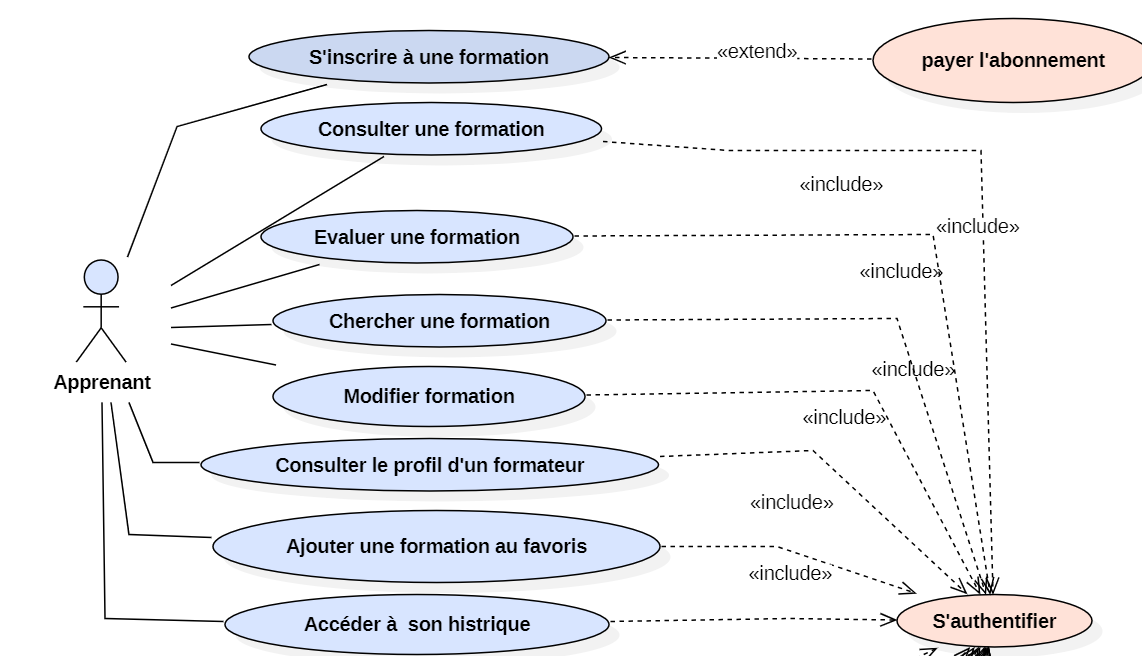
\includegraphics[width=15cm]{Figures/apprenant.PNG}
    \caption{ Diagramme de cas d’utilisation d'apprenant}
    %\label{fig:my_label} %Optional (If you want to reference the figure in later chapters)
\end{figure}

\begin{figure}[H] 
    \centering
    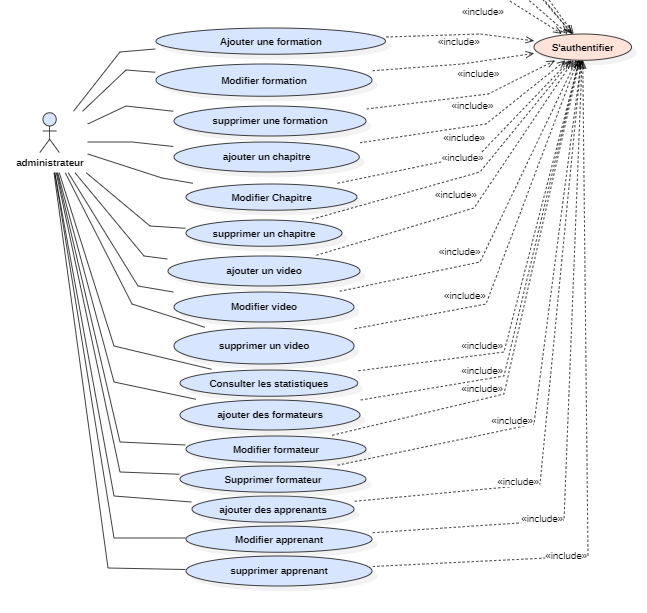
\includegraphics[width=13cm]{Figures/administrateur.PNG}
    \caption{ Diagramme de cas d’utilisation d'administrateur}
    %\label{fig:my_label} %Optional (If you want to reference the figure in later chapters)
\end{figure}


\subsection{Description textuelle de cas d’utilisation: }
\begin{table}[h!]
\centering
\begin{tabular}{| m{7cm} | m{7cm} |}
\hline
\multicolumn{2}{|c|}{\textbf{UC 1:} Payer l'abonnement d'une formation} \\ \hline
\textbf{Acteurs} &  Utilisateur \\ \hline
\textbf{But} &   Permettre à un utilisateur d'accéder à une formation disponible sur la plateforme et voir les videos \\ \hline
 \textbf{Préconditions} 
& 
\textbf{Postconditions} \\ \hline
- S'authentifier. & - voir les videos\\ \hline
\textbf{Scénario Principal} & \textbf{Scénario Alternatif}
\\ \hline
\begin{enumerate}
    \item S'authentifier.
    \item Naviguer vers la page de la formation.
    \item Choisir la formation.
    \item Clique sur "S'inscrire".
    \item Effectuer le paiement.
    \item Si le paiement est autoris.
    \item Client est redirigé vers la page de confirmation de paiement.
\end{enumerate} & 
\begin{enumerate}
    \item S'authentifier.
    \item Naviguer vers la page de la formation.
    \item Choisir la formation.
    \item Clique sur "S'inscrire".
    \item Effectuer le paiement.
    \item Si le paiement n'est pas autorisé.
    \item Client est redirigé vers la page d’erreur.
\end{enumerate}
\\ \hline
\end{tabular}
\caption{Description Textuelle du Cas d'Utilisation "Payer l'abonnement d'une formation"}
\label{tab:use_case_description}
\end{table}


\begin{table}[h!]
    \centering
    \begin{tabular}{| m{7cm} | m{7cm} |}
    \hline
    \multicolumn{2}{|c|}{\textbf{UC 2:} Ajouter une formation} \\ \hline
    \textbf{Acteurs} &  Administrateur \\ \hline
    \textbf{But} &   Permettre à un administrateur d'ajouter une formation à la plateforme avec ces chapitres et ces vidéos \\ \hline
     \textbf{Préconditions} 
    & 
    \textbf{Postconditions} \\ \hline
    - S'authentifier. & - \\ \hline
    \textbf{Scénario Principal} & \textbf{Scénario Alternatif}
    \\ \hline
    \begin{enumerate}
        \item S'authentifier.
        \item Naviguer vers la page d'ajout de formation.
        \item remplir les informations nécessaire pour la formation
        \item Ajouter les chapitres.
        \item Ajouter les vidéos.
        \item Clique sur le bouton "Enregistrer".
        \item Un message de confirmation est affiché
    \end{enumerate} & 
    \begin{enumerate}
        \item S'authentifier.
        \item Naviguer vers la page d'ajout de formation.
        \item remplir les informations nécessaire pour la formation
        \item Ajouter les chapitres.
        \item Ajouter les vidéos.
        \item Clique sur le bouton "Enregistrer".
        \item un message d'erreur spécifiant les champs incorrects ou manquants est affiché.
    \end{enumerate}
    \\ \hline
    \end{tabular}
    \caption{Description Textuelle du Cas d'Utilisation "Ajouter une formation"}
    \label{tab:use_case_description}
    \end{table}

    
\begin{table}[h!]
    \centering
    \begin{tabular}{| m{7cm} | m{7cm} |}
    \hline
    \multicolumn{2}{|c|}{\textbf{UC 3:} Ajouter un chapitre} \\ \hline
    \textbf{Acteurs} &  Administrateur \\ \hline
    \textbf{But} &   Permettre à un administrateur d'ajouter un chapitre à une formation existante \\ \hline
     \textbf{Préconditions} 
    & 
    \textbf{Postconditions} \\ \hline
    - S'authentifier. & - \\ \hline
    \textbf{Scénario Principal} & \textbf{Scénario Alternatif}
    \\ \hline
    \begin{enumerate}
        \item S'authentifier.
        \item Naviguer vers la page des formations.
        \item remplir les informations nécessaire pour le chapitre.
        \item Ajouter les vidéos.
        \item Clique sur le bouton "Enregistrer".
        \item Un message de confirmation est affiché
    \end{enumerate} & 
    \begin{enumerate}
        \item S'authentifier.
        \item Naviguer vers la page des formations.
        \item remplir les informations nécessaire pour le chapitre.
        \item Ajouter les vidéos.
        \item Clique sur le bouton "Enregistrer".
        \item Un message d'erreur spécifiant les champs incorrects ou manquants est affiché.
    \end{enumerate}
    \\ \hline
    \end{tabular}
    \caption{Description Textuelle du Cas d'Utilisation "Ajouter un chapitre"}
    \label{tab:use_case_description}
    \end{table}

  
    \begin{table}[h!]
        \centering
        \begin{tabular}{| m{7cm} | m{7cm} |}
        \hline
        \multicolumn{2}{|c|}{\textbf{UC 4:} Ajouter un apprenant} \\ \hline
        \textbf{Acteurs} &  Administrateur \\ \hline
        \textbf{But} &   Permettre à un administrateur d'ajouter un apprenant pour qu'il peut s'authentifier à la plateforme. \\ \hline
         \textbf{Préconditions} 
        & 
        \textbf{Postconditions} \\ \hline
        - S'authentifier. & - \\ \hline
        \textbf{Scénario Principal} & \textbf{Scénario Alternatif}
        \\ \hline
        \begin{enumerate}
            \item S'authentifier.
            \item Naviguer vers la page des apprenants.
            \item remplir les informations nécessaire pour l'apprenant.
            \item Clique sur le bouton "Enregistrer".
            \item Un message de confirmation est affiché
        \end{enumerate} & 
        \begin{enumerate}
            \item S'authentifier.
            \item Naviguer vers la page des apprenants.
            \item remplir les informations nécessaire pour l'apprenant.
            \item Clique sur le bouton "Enregistrer".
            \item Un message d'erreur spécifiant les champs incorrects ou manquants est affiché.
        \end{enumerate}
        \\ \hline
        \end{tabular}
        \caption{Description Textuelle du Cas d'Utilisation "Ajouter un apprenant"}
        \label{tab:use_case_description}
        \end{table}
    